\documentclass[14pt, hyperref = {colorlinks}]{beamer}
\usepackage[T2A]{fontenc}
\usepackage[utf8]{inputenc}
\usepackage[english,russian]{babel}
\usepackage[colorlinks]{hyperref}
\usepackage{amssymb,amsfonts,amsmath,mathtext}
\usepackage{cite,enumerate,float,indentfirst}


\usepackage{xmpmulti}
\usepackage{gensymb} % для обозачения град
%\usefonttheme{structurebold}     % Font theme: serif
%\usepackage{ccfonts}     % Font family: Concrete Math
%\usepackage[T1]{fontenc} % Font encoding: T1
\DeclareMathOperator{\sinc}{sinc}

\hypersetup{
	colorlinks=true,
	linkcolor=blue,
	filecolor=magenta,      
	urlcolor=cyan,
}

\usetheme{Boadilla}
\usecolortheme{seahorse}
%\usefonttheme[onlymath]{serif}

\setbeamercolor{footline}{fg=blue}
\setbeamertemplate{footline}{
	\leavevmode%
	\hbox{%
		\begin{beamercolorbox}[wd=.333333\paperwidth,ht=2.25ex,dp=1ex,center]{}%
			А.Е. Требушинин
		\end{beamercolorbox}%
		\begin{beamercolorbox}[wd=.333333\paperwidth,ht=2.25ex,dp=1ex,center]{}%
			Новосибирск, 2019
		\end{beamercolorbox}%
		\begin{beamercolorbox}[wd=.333333\paperwidth,ht=2.25ex,dp=1ex,right]{}%
			Стр. \insertframenumber{} из \inserttotalframenumber \hspace*{2ex}
	\end{beamercolorbox}}%
	\vskip0pt%
}

\newcommand{\itemi}{\item[\checkmark]}

\title{\small{Разработка рентгенооптических трактов экспериментальных станций первой очереди проекта ЦКП «СКИФ»}}

\author{\small{%
		\emph{Докладчик:}~Требушинин~А.Е.\\%
		\emph{Руководитель:}~к.ф.-м.н. Ракшун~Я.В.}\\%
	\vspace{30pt}%
  	ИЯФ СО РАН
	\vspace{-15pt}%
}

\date{
\includegraphics[width=0.1\linewidth]{pic/logo.jpg} \hspace{20pt}
	
\includegraphics[width=0.2\linewidth]{pic/SKIFlogo.png}\\
	
	\vspace{5pt}% 
	\small{Новосибирск, 2019}}

\begin{document}

\maketitle

\small
\begin{frame}\label{r3}
\frametitle{Карта ускорительных центров}
\vspace{-20pt}
\begin{figure}[h]
	\center{\includegraphics[width=1.0\linewidth]{pic/map.png}}	
	\raggedright\tiny{Жёлтым цветом обозначены центры синхротронного излучения}
\end{figure}
\end{frame}

\iffalse
\small
\begin{frame}
\frametitle{Задачи, решаемые на синхротроне}\label{t1}
\begin{center}
	\begin{itemize}
		\item Белковая кристаллография		 
		\item Рентгеновская микроскопия, радиография, томография
		
	\end{itemize}
\end{center}
\end{frame}
\fi

\small
\begin{frame}
\frametitle{Цель}\label{t1}
\begin{center}
	\large{Создание проекта экспериментальных стаций первой очереди ЦКП <<СКИФ>>}
\end{center}
\end{frame}

\small
\begin{frame}
\frametitle{СКИФ \centering{\small{Сибирский Кольцевой Источник Фотонов}}}\label{t1}
\vspace{-20pt}
\begin{figure}[h]
	\hfill
	\center{}
	\begin{minipage}[h]{0.99\linewidth}
		\center{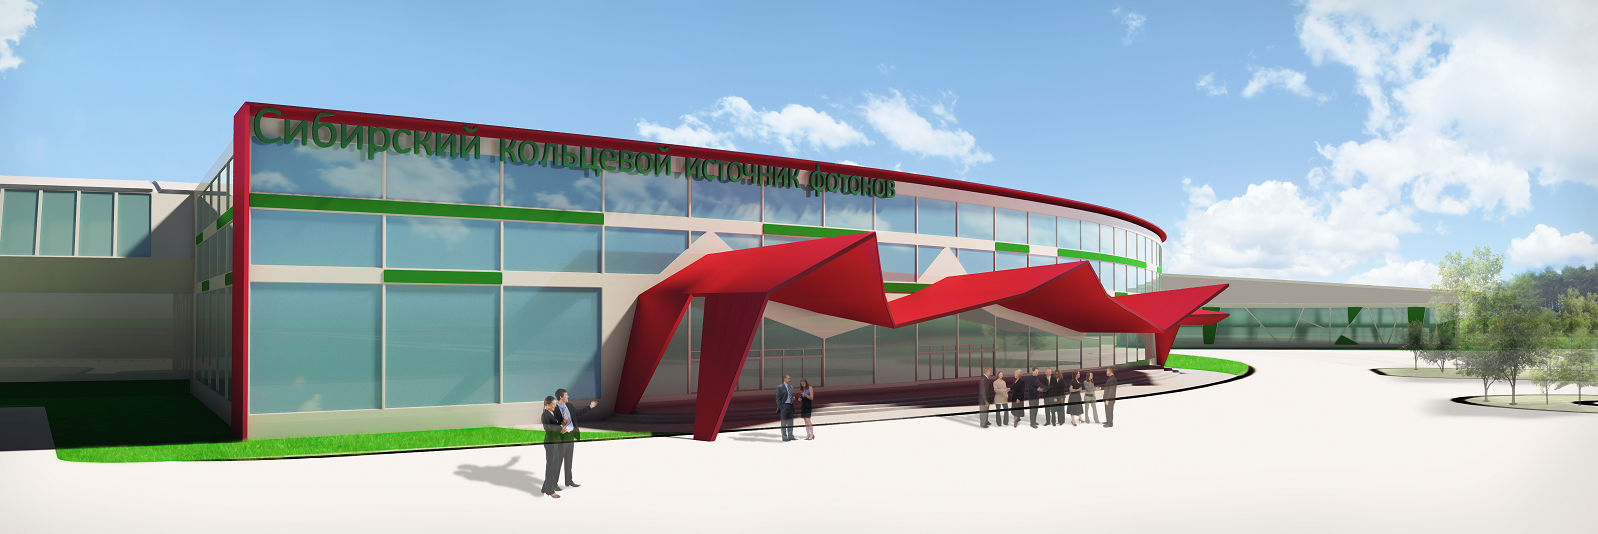
\includegraphics[width=0.99\linewidth]{pic/SKIF_1_2.png}}
		%https://portal.slac.stanford.edu
	\end{minipage}
\end{figure}
\vspace{-20pt}
\begin{table}[h]
	\begin{tabular}{|c|c|c|c|c|c|}
		\hline
		\hline
		\rule{0pt}{3ex}   $\mathnormal{E, [GeV]}$ & $\mathnormal{I, [mA]}$ & $\mathnormal{C, [m]}$& $\mathnormal{\epsilon_x, [pm rad]}$ & $\mathnormal{\epsilon_y, [pm rad]}$ & $\mathnormal{N}$				\\ \hline
		\rule{0pt}{3ex}   $\mathnormal{3}$		  & $\mathnormal{400}    $ & $\mathnormal{476}$   &$\mathnormal{90}$        		    & $\mathnormal{60}$  			      & $\mathnormal{30}$     \\ \hline
	\end{tabular}
\end{table}
\end{frame}

\small
\begin{frame}
\frametitle{Схема ЦКП <<СКИФ>>}\label{t1}
\vspace{-10pt}
\begin{figure}[h]
	\center{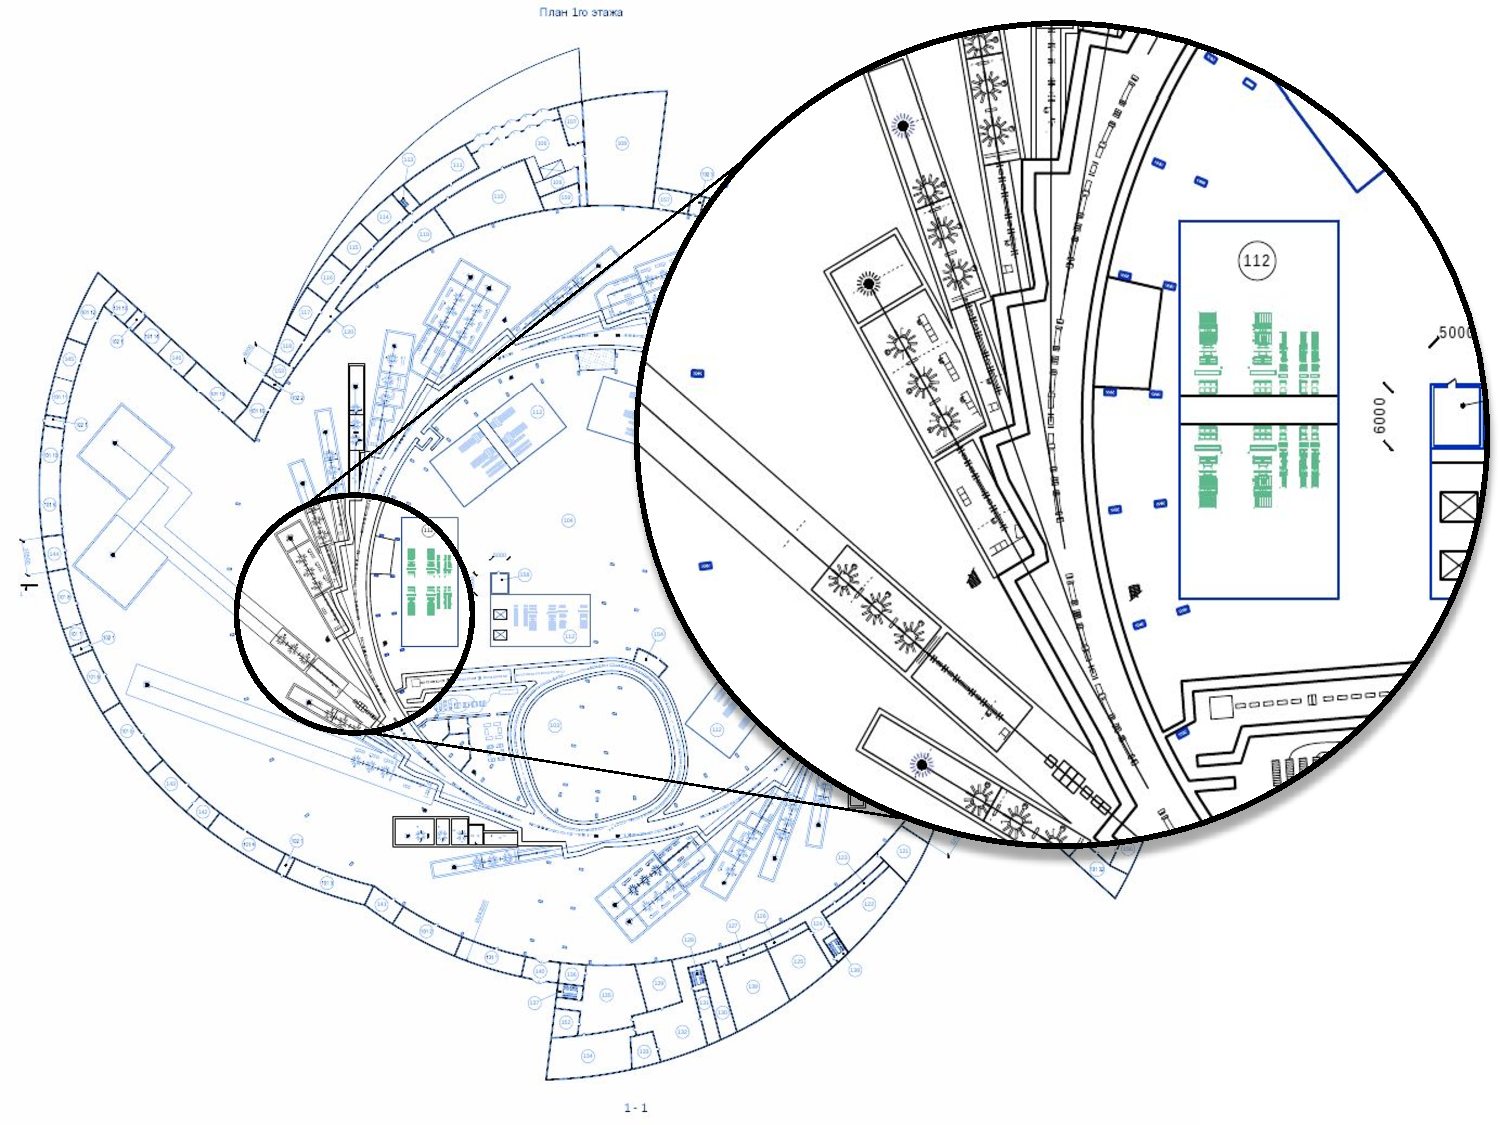
\includegraphics[width=0.95\linewidth]{pic/outline.pdf}}	
\end{figure}
\end{frame}

\small
\begin{frame}
\frametitle{Задачи}\label{t1}
\begin{center}
\begin{itemize}
	\item Моделирование \textbf{вставных устройств} \\(ондуляторы)
  	\item Оптимизация \textbf{оптических элементов} \\(апертуры, монохроматоры, фокусирующие зеркала)
  	\item Создание \textbf{среды для обмена информацией} по проектированию
	\item Координация работы между исследовательскими группами разных институтов (ИЯФ СО РАН, ИК СО РАН, ИГиЛ СО РАН, ИГМ СО РАН)
\end{itemize}
\end{center}
\end{frame}



\small
\begin{frame}
\frametitle{План презентации}\label{t1}
\begin{center}
		\begin{itemize}
		\item Схема работы <<Оптической группы>> ЦКП СКИФ
		\item Принципиальные основы кода для расчёта синхротронного излучения SRW
		\item Обзор типовых ондуляторов для <<СКИФ>>
		\item Расчёт оптической схемы станции 1-1
		\item Расчёт ондулятора с корректирующими катушками для станции 1-4 
	\end{itemize}
\end{center}
\end{frame}

\iffalse
\small
\begin{frame}
\frametitle{Окружности и прямые}\label{t1}
\begin{figure}[h]
	\center{Синхротронный источник}
	\begin{minipage}[h]{0.50\linewidth}
		\center{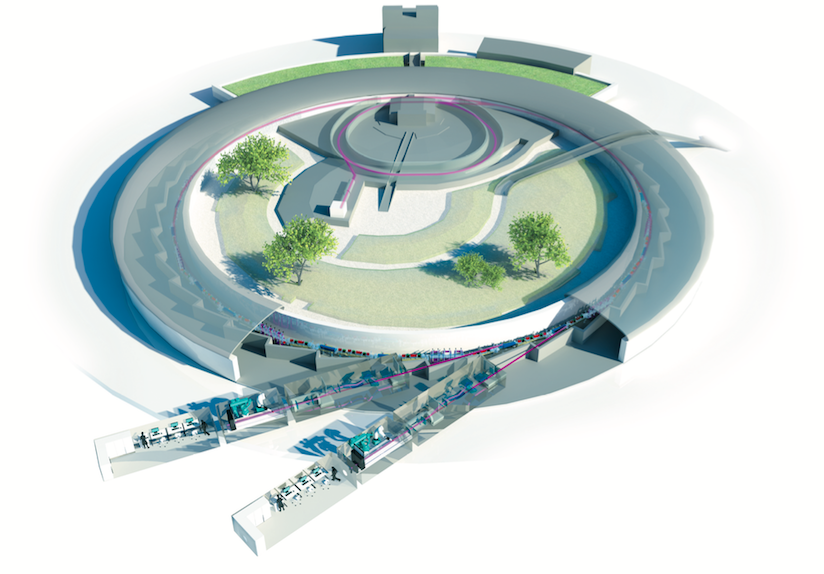
\includegraphics[width=0.99\linewidth]{pic/synchrotron.png}}
		%http://www.irtnanoelec.fr
	\end{minipage}

	\hfill
	\center{Лазер на свободный электронах}
	\begin{minipage}[h]{0.50\linewidth}
		\center{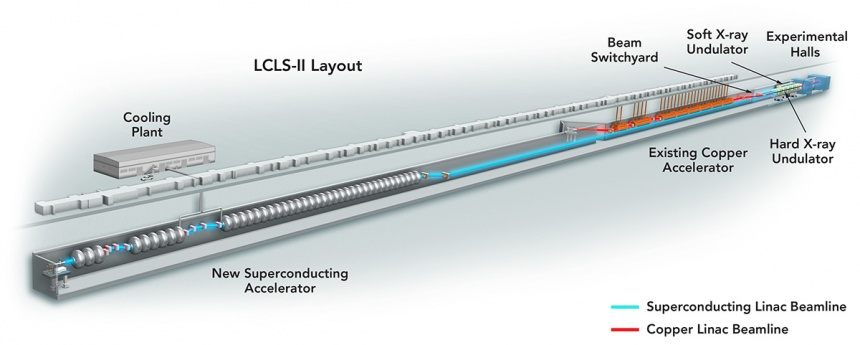
\includegraphics[width=0.99\linewidth]{pic/lcls.jpg}}
		%https://portal.slac.stanford.edu
	\end{minipage}
	\end{figure}
	\raggedright\tiny{\href{http://www.irtnanoelec.fr}{ссылка на рисунок сверху}}\\
	\raggedright\tiny{\href{https://portal.slac.stanford.edu/sites/conf_public/lclsiihe2018/PublishingImages/Forms/AllItems.aspx}{ссылка на рисунок снизу}}
\end{frame}
\fi

\small
\begin{frame}
\frametitle{Оптическая группа ЦКП <<СКИФ>>}\label{t1}
\vspace{-20pt}
\begin{figure}[h]
	\center{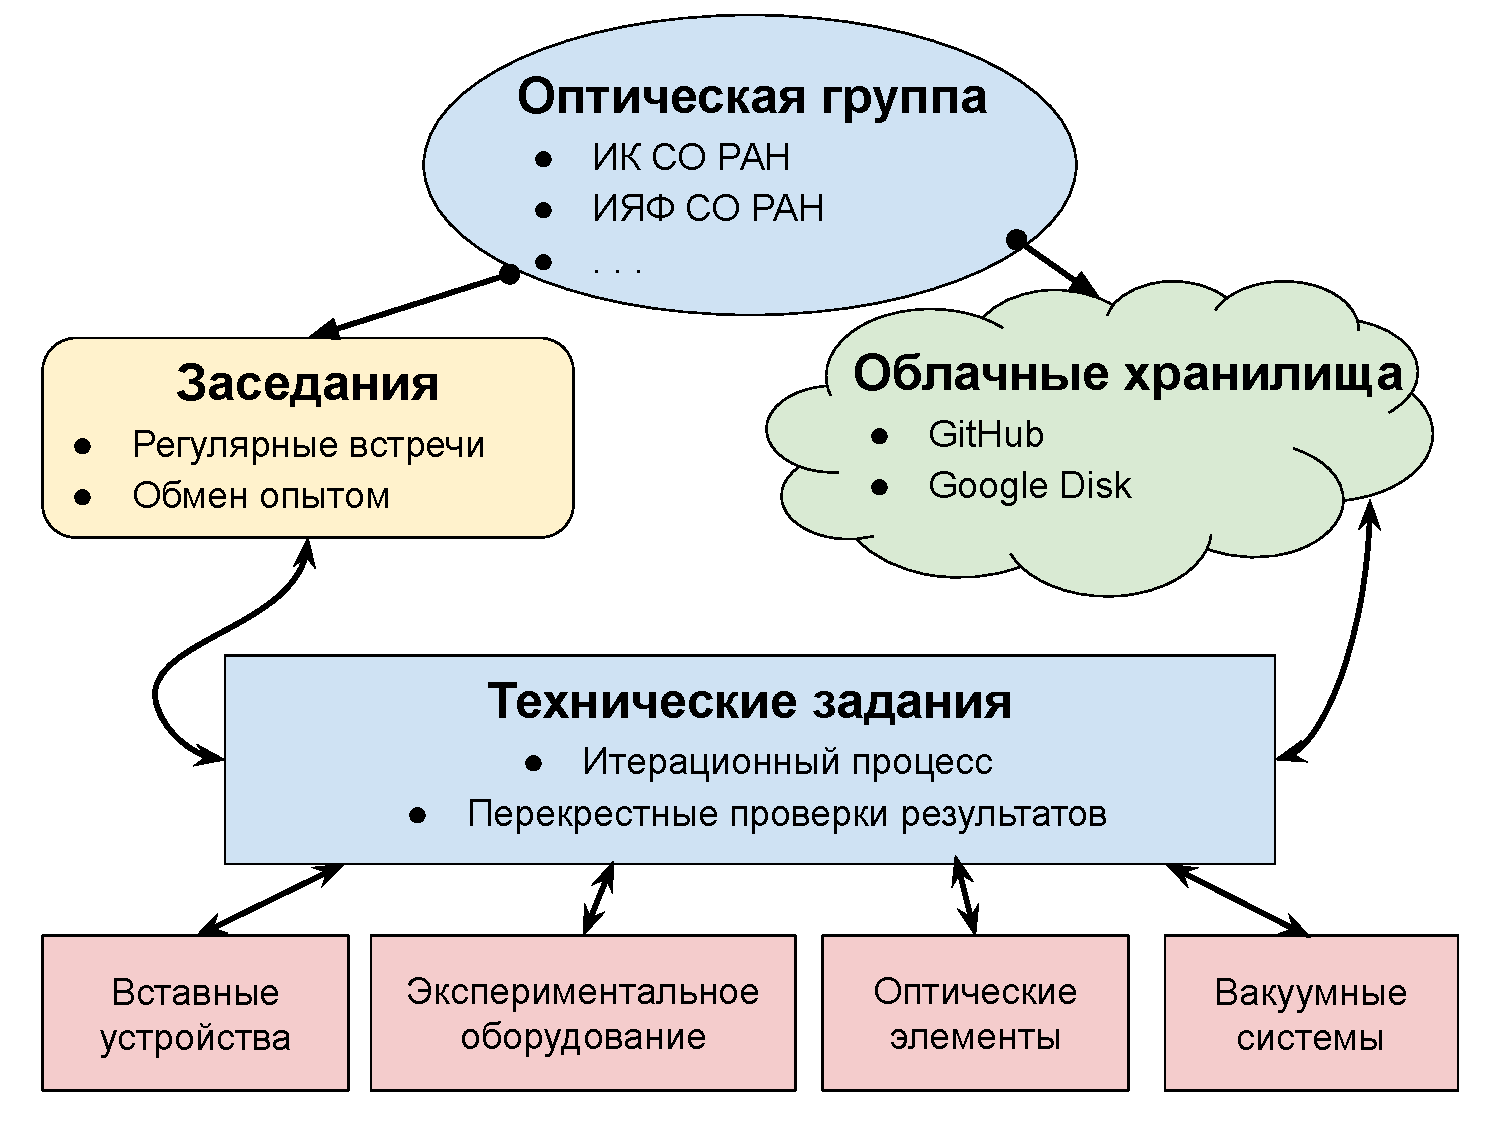
\includegraphics[width=0.8\linewidth]{pic/optgr.pdf}}
\end{figure}
\tiny{\textit{@Andrei Trebushinin ссылка на \href{https://github.com/TrebAndrew/thesis_andrei.git}{GitHub}}}
\end{frame}

\small
\begin{frame}
\frametitle{SRW. Среда моделирования}\label{t1}
SRW --- Synchrotron Radiation Workshop. Код для моделирования оптических систем.
$\mathnormal{r\omega}$-пространство, ближняя зона.\\
\begin{itemize}
	\item Вставные устройства:\\
\end{itemize}
	\hspace{25pt}$\mathnormal{\vec{\widetilde{E}}_{\bot}(\vec{r}_0, \omega) = 
	\cfrac{i\omega e}{c}\displaystyle\int\limits_{-\infty}^{\infty} dt'\bigg[\cfrac{\vec{\beta} - \vec{n}}{|\vec{r}_0 - \vec{r'}_0(t')|} - \cfrac{ic}{\omega}\cfrac{\vec{n}}{|\vec{r}_0 - \vec{r'}_0(t')|^2}\bigg]\times}$\\
	\hspace{195pt}$\mathnormal{\exp\bigg[i\bigg(t' + \cfrac{|\vec{r}_0 - \vec{r'}_0(t')|}{c}\bigg)\bigg]}$

\begin{itemize}	
	\item Фурье оптика:\\
	\centering
	\vspace{-10pt}
	$\mathnormal{g_2(x_2, y_2) = \displaystyle\int\limits_{-\infty}^{\infty}\displaystyle\int\limits_{-\infty}^{\infty}
		g_1(\eta, \xi) h(x_2 - \eta, y_2 - \xi)}d\eta d\xi$ \\
	\vspace{-6pt}
	$\Updownarrow$\\
	\vspace{6pt}
	$\mathnormal{G_2(f_x, f_y) = G_1(f_x, f_y)H(f_x, f_y)}$
\end{itemize}
\tiny{\textit{@Oleg Chubar ссылка на \href{https://github.com/ochubar/SRW.git}{GitHub}}}
\end{frame}
%\vec{\widetilde{E}}_{\bot}(\vec{r}_0, \omega) =
%\cfrac{i\omega e}{c}\displaystyle\int\limits_{-\infty}^{\infty} dt'\bigg[\cfrac{\vec{\beta} - \vec{n}}{|\vec{r}_0 - \vec{r'}_0(t')|}-\cfrac{ic}{\omega}\cfrac{\vec{n}}{|\vec{r}_0 - \vec{r'}_0(t')|}\bigg]\\
%\exp[i\bigg(t' + \cfrac{|\vec{r}_0 - \vec{r'}_0(t')|}{c}\bigg)]


\small
\begin{frame}
\frametitle{Ондулятор --- интерференционное устройство}\label{t1}
\begin{figure}[h]
		\center{$\mathnormal{n \lambda_{ph} = s_{ph} - \lambda_u \cos\theta}$}\hspace{10pt}$\longrightarrow$\hspace{10pt}
		{$\mathnormal{\lambda_{ph} = \cfrac{\lambda_{u}}{2n\gamma^2 K}\bigg(1 + \cfrac{K^2}{2} + \gamma^2\theta^2\bigg)}$}
		%\\
%		$K = \cfrac{eB_0 \lambda}{2\pi m_ek_w}$
		%\vspace{-20pt}
		\center{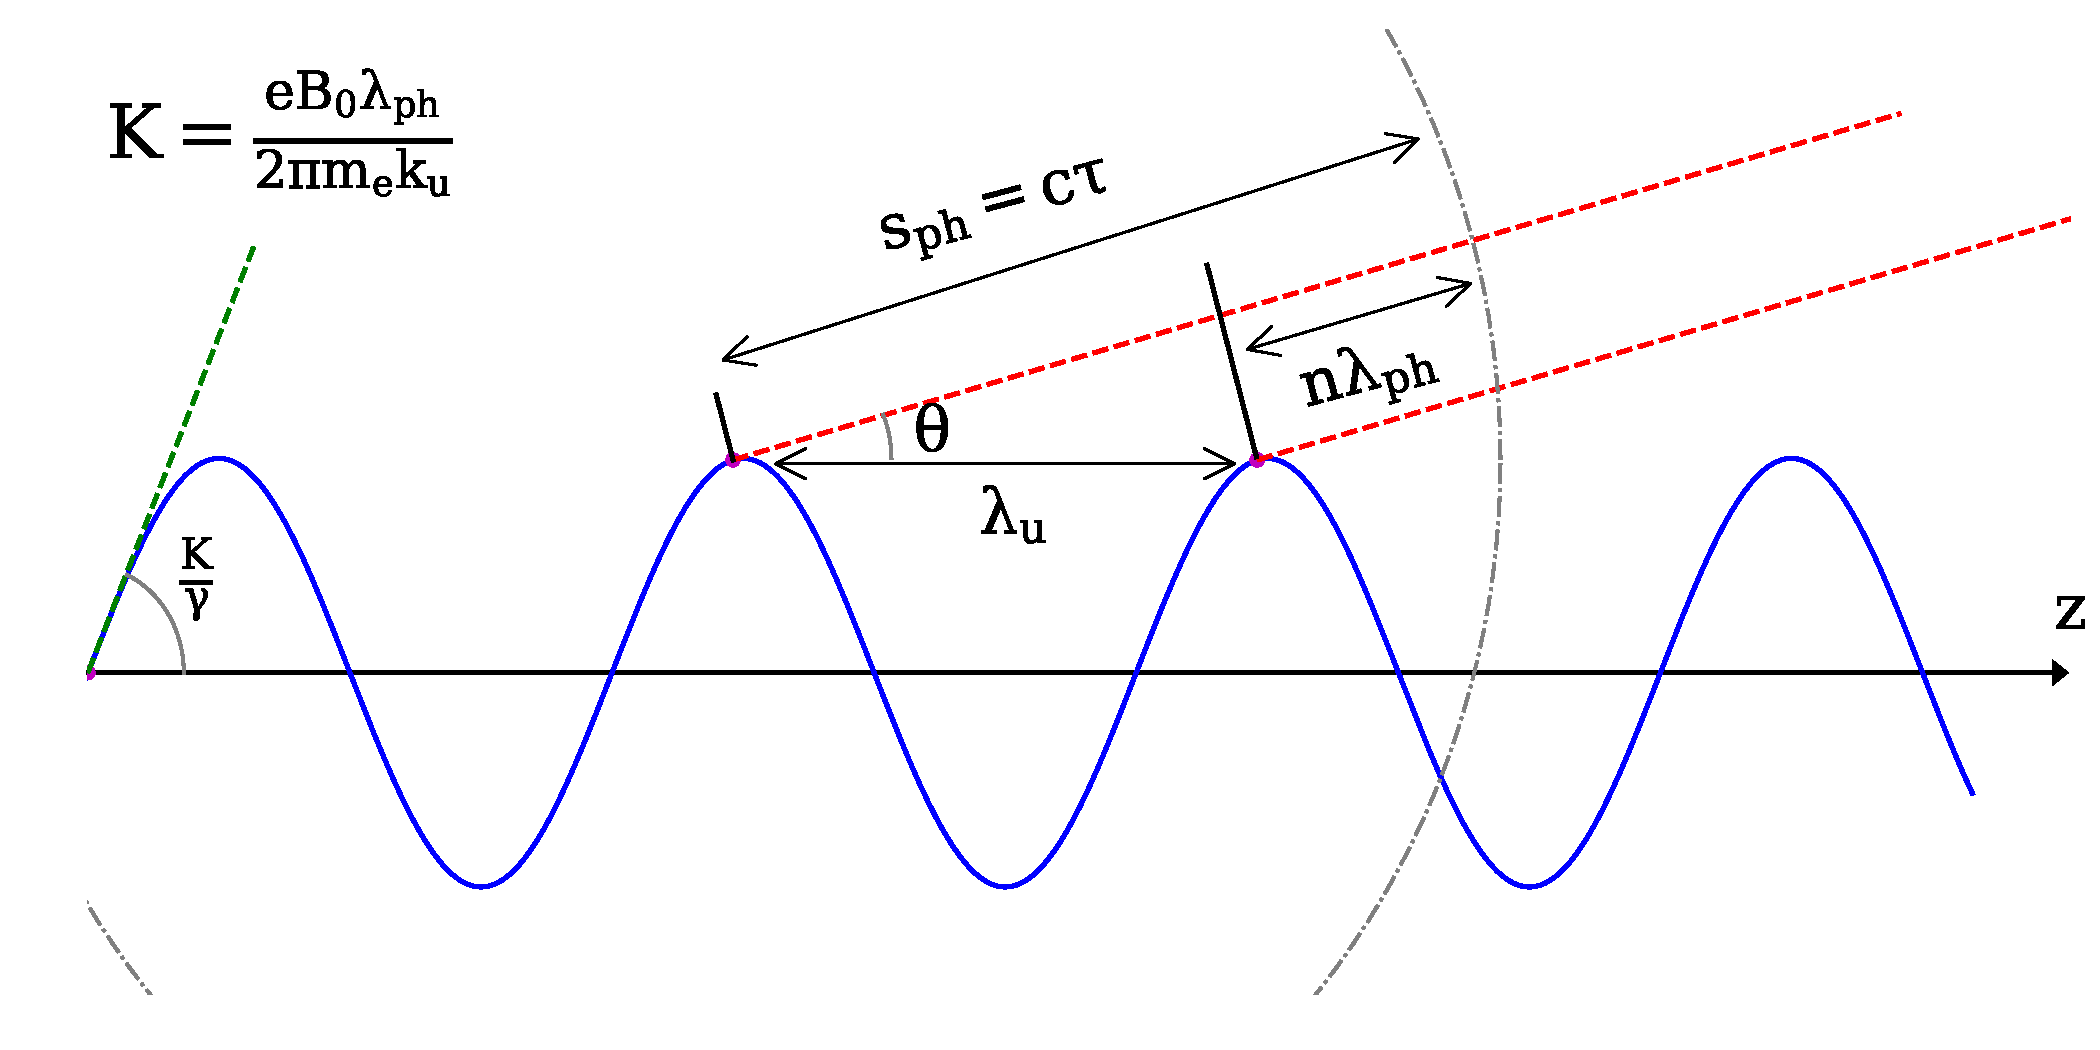
\includegraphics[width=0.99\linewidth]{pic/traj.pdf}}
\end{figure}
 \end{frame}

\small
\begin{frame}
\frametitle{Стандартные ондуляторы для СКИФ}\label{t1}
\vspace{-10pt}
\begin{figure}[h]
	\begin{minipage}[h]{0.49\linewidth}
		\raggedright{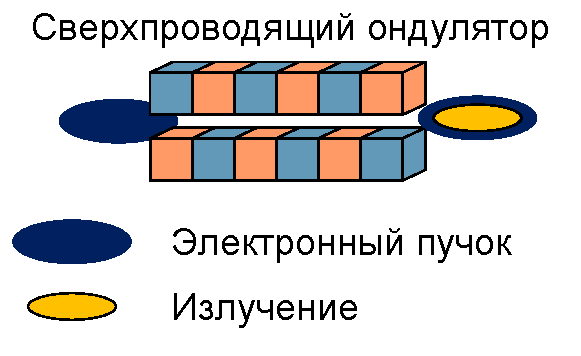
\includegraphics[width=0.99\linewidth]{pic/sim_und.pdf}}
	\end{minipage}
	\begin{minipage}[h]{0.49\linewidth}
	\vspace{10pt}
	\begin{table}[h]
		\begin{tabular}{|c|c|c|c|}
			\hline\hline
			\rule{0pt}{3ex}$\mathnormal{B, [T]}$      & $\mathnormal{0.7 - 1.5}$   \\ \hline
			\rule{0pt}{3ex}$\mathnormal{L, [m]}$ 	  &  $\mathnormal{3}$        \\ \hline
			\rule{0pt}{3ex}$\mathnormal{d, [mm]}$     & $\mathnormal{15 - 20}$     \\ \hline
			\rule{0pt}{3ex}$\mathnormal{N}$           & $\mathnormal{\geq 120}$ \\ \hline
			\rule{0pt}{3ex}Фазовая ошибка &$\mathnormal{\leq 2^{\circ}}$  \\
			\hline
		\end{tabular}
	\end{table}
	\end{minipage}
\end{figure}
\vspace{-20pt}
\begin{table}[h]
	\begin{tabular}{|c|c|c|c|c|}
		\hline
		\hline
		\rule{0pt}{3ex}   $\mathnormal{E, [GeV]}$ & $\mathnormal{I, [mA]}$ & $\mathnormal{\beta_x, [m]}$ & $\mathnormal{\beta_{y}, [m]}$&\\ \hline
		\rule{0pt}{3ex}   $\mathnormal{3}$		 & $\mathnormal{400}    $ & $\mathnormal{12.48}$        & $\mathnormal{1.99}$  &   \\ \hline
		\hline	
		\rule{0pt}{3ex}   $\mathnormal{\sigma_x, [m]}$ & $\mathnormal{\sigma_{x'}, [rad]}$ & $\mathnormal{\sigma_y, [m]}$     & $\mathnormal{\sigma_{y'}, [rad]}$ & $\mathnormal{\Delta E / E}$      \\ \hline
		\rule{0pt}{3ex}   $\mathnormal{33.0 \times 10^{-6}}$  & $\mathnormal{2.65 \times 10^{-6}}$  &  $\mathnormal{8.6 \times 10^{-7}}$ & $\mathnormal{5.0 \times 10^{-7}}$   & $\mathnormal{8.6 \times 10^{-4}}$ \\
		\hline
	\end{tabular}
\end{table}
\end{frame}

\small
\begin{frame}
\frametitle{Расчёт станции 1-1. Тепловые нагрузки}\label{t1}
\vspace{-10pt}
\begin{figure}[h]
	\begin{minipage}[h]{0.49\linewidth}
		\raggedright{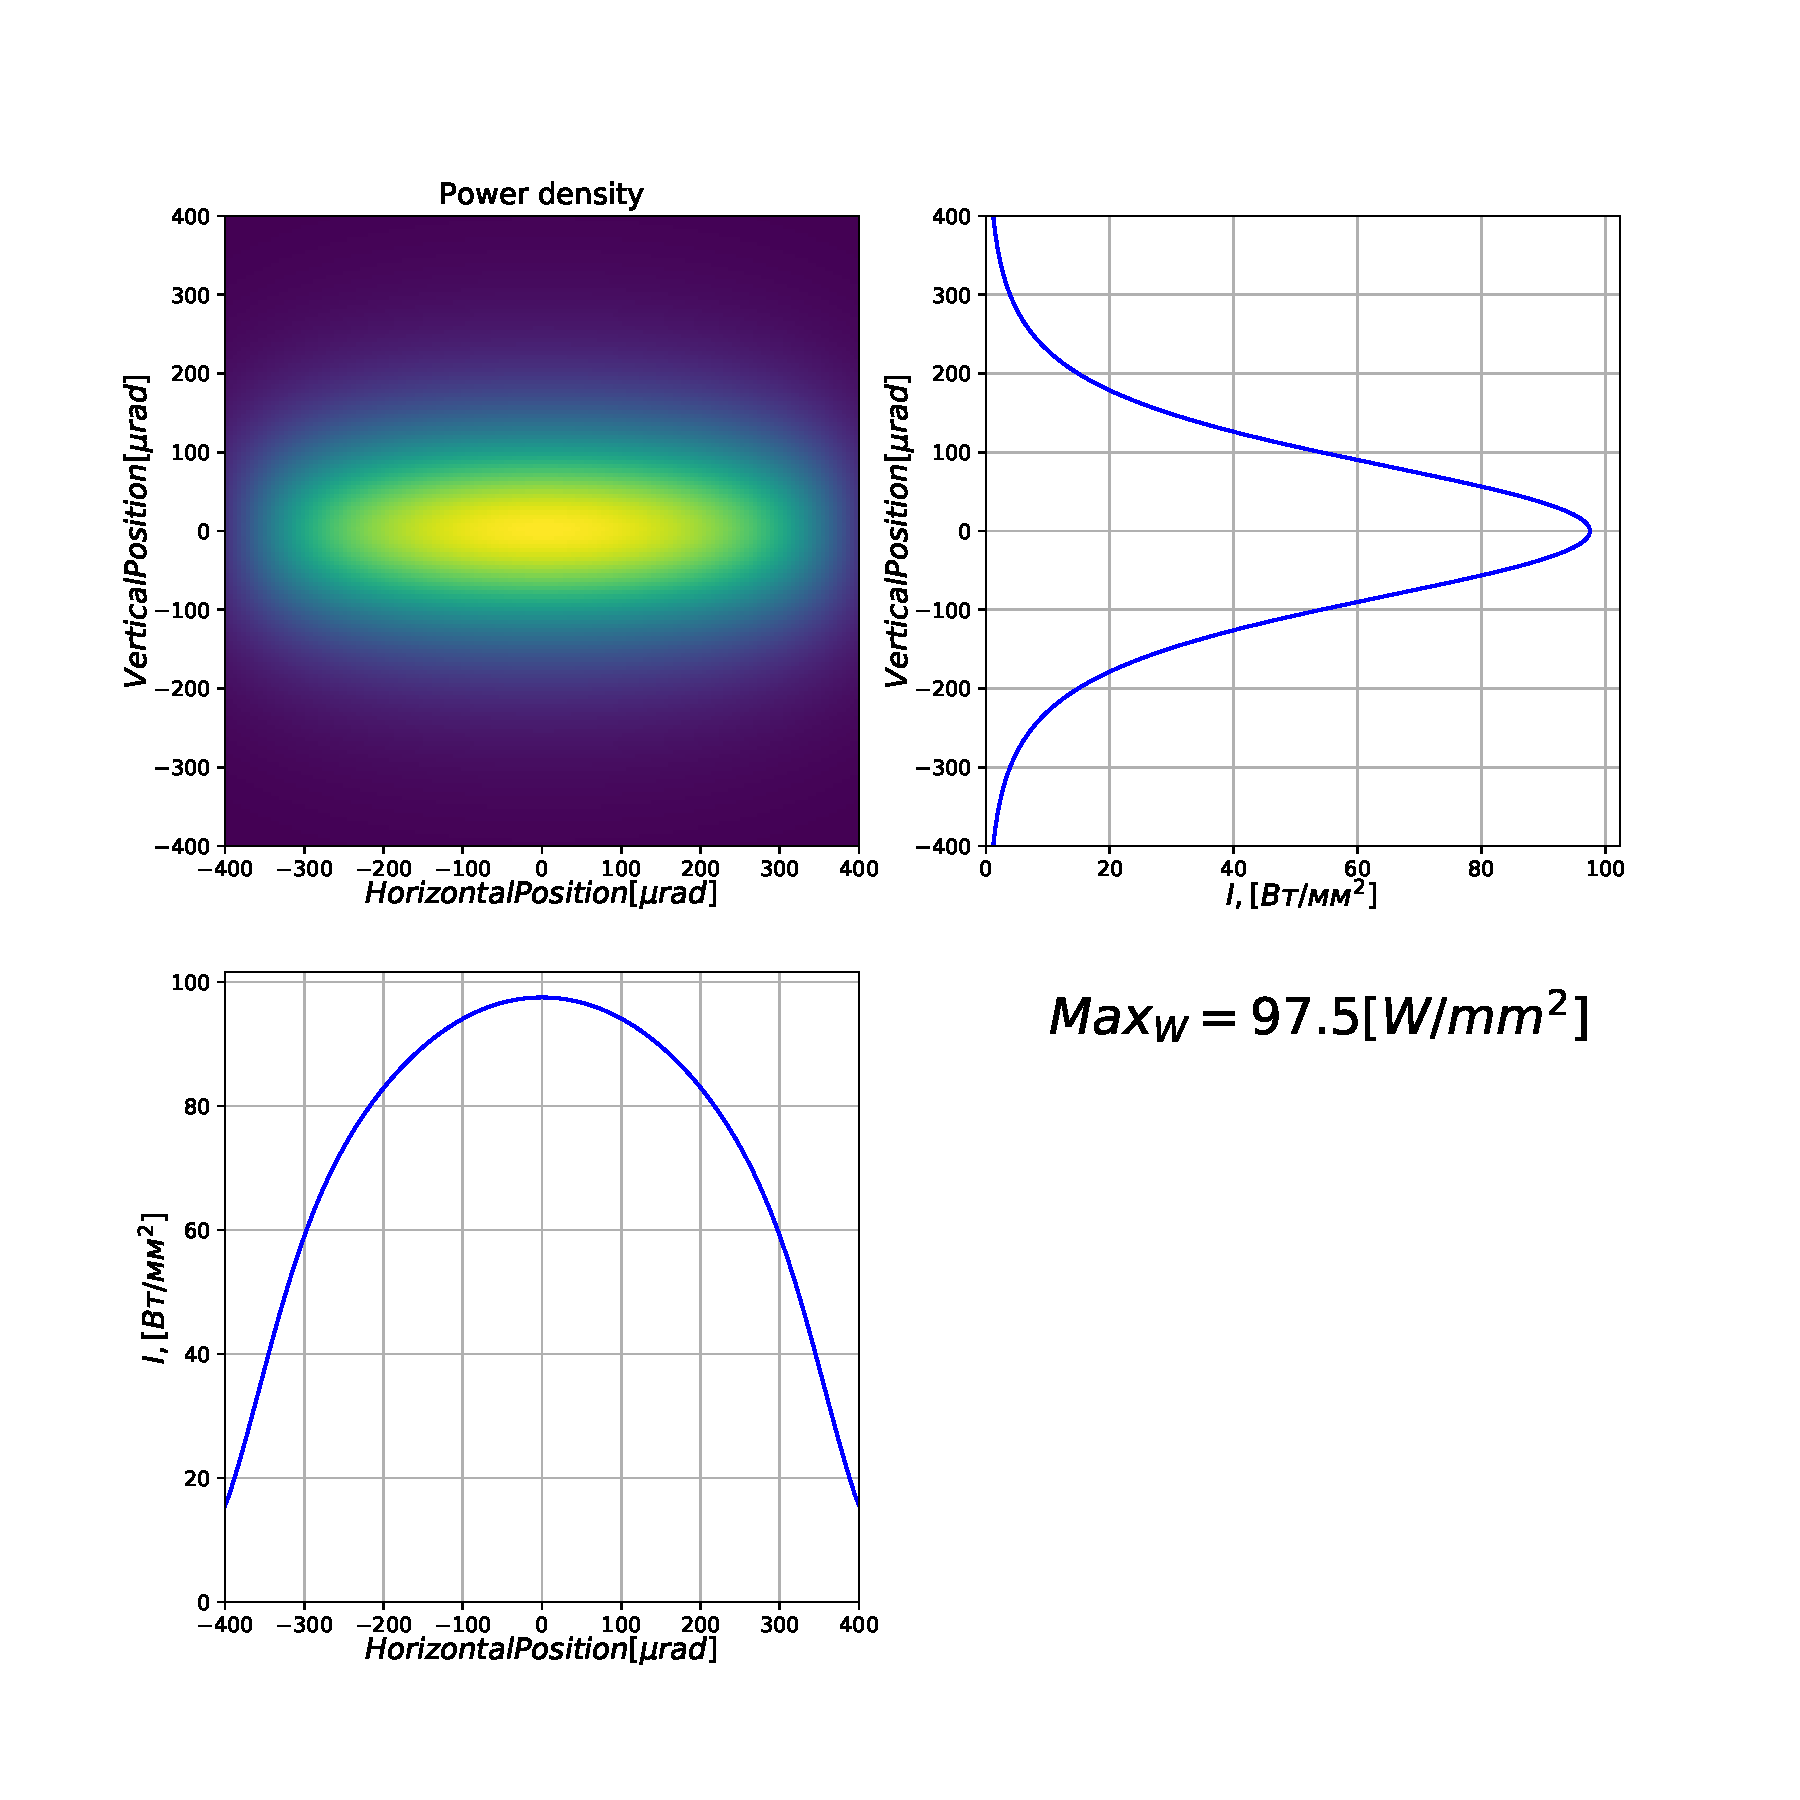
\includegraphics[width=1.1\linewidth]{pic/power_dens.pdf}}
	\end{minipage}
	\begin{minipage}[h]{0.49\linewidth}
		\raggedleft{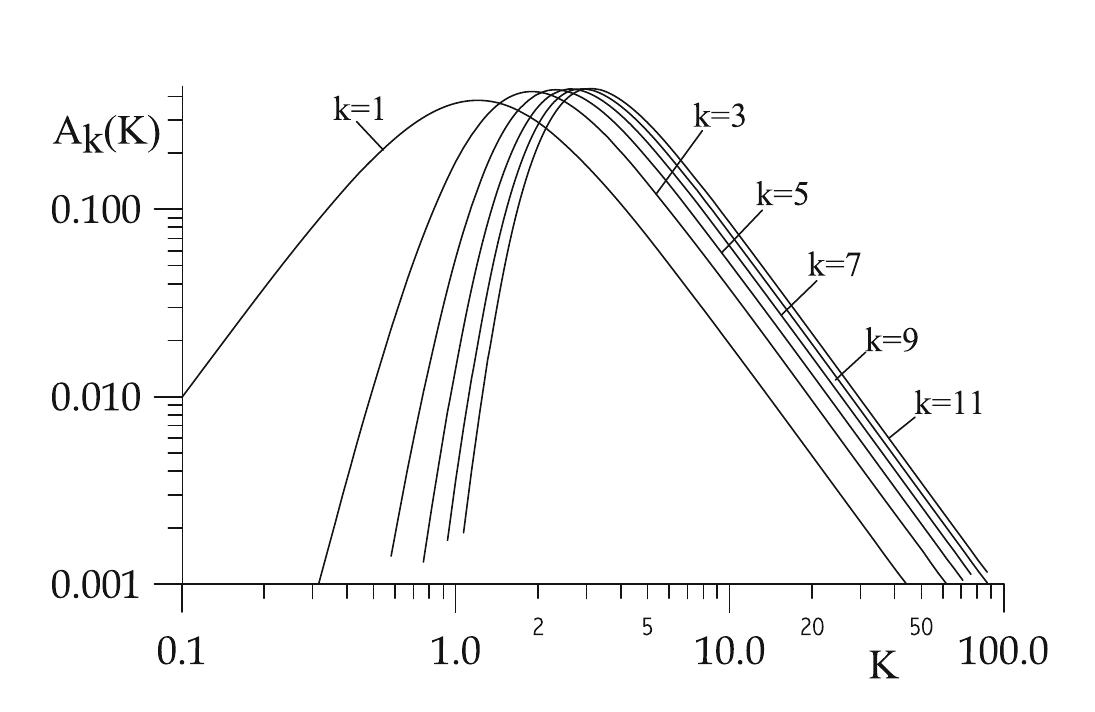
\includegraphics[width=0.9\linewidth]{pic/AA_harm.png}}
		\begin{minipage}[h]{0.99\linewidth}
			%\vspace{-90pt}	
			\tiny
			\vspace{10pt}	
			\begin{table}[h]
				\begin{tabular}{|c|c|c|c|c|}
					\hline\hline
					\rule{0pt}{3ex}$\mathnormal{B(K), [T]}$   & $\mathnormal{1.36(2.29)}$   \\ \hline
					\rule{0pt}{3ex}$\mathnormal{L, [m]}$ 	  & $\mathnormal{2.3}$          \\ \hline
					\rule{0pt}{3ex}$\mathnormal{d, [mm]}$     & $\mathnormal{18}$    		\\ \hline
					\rule{0pt}{3ex}Фазовая ошибка             &$ \mathnormal{\leq 3^{\circ}}$  \\ \hline
					\rule{0pt}{3ex}Гармоники	              & $\mathnormal{11, 13, 17, 23}$  \\
					\hline
				\end{tabular}
			\end{table}
		\end{minipage}
	\end{minipage}
\end{figure}

%\tiny{\textit{@Andrei Trebushinin ссылка на \href{https://github.com/TrebAndrew/thesis_andrei.git}{GitHub}}}
\end{frame}

\iffalse
	\begin{minipage}[h]{0.24\linewidth}
	%\vspace{-90pt}	
	\tiny
	\begin{table}[h]
		\begin{tabular}{|c|c|c|c|c|}
			\hline\hline
			\rule{0pt}{3ex}$\mathnormal{B(K), [T]}$   & $\mathnormal{1.36(2.29)}$   \\ \hline
			\rule{0pt}{3ex}$\mathnormal{L, [m]}$ 	  & $\mathnormal{2.3}$          \\ \hline
			\rule{0pt}{3ex}$\mathnormal{d, [mm]}$     & $\mathnormal{18}$    		\\ \hline
			\rule{0pt}{3ex}Фазовая ошибка             &$ \mathnormal{\leq 3^{\circ}}$  \\ \hline
			\rule{0pt}{3ex}Гармоники	              & $\mathnormal{11, 13, 17, 23}$  \\
			\hline
		\end{tabular}
	\end{table}
\end{minipage}
\fi

\small
\begin{frame}
\frametitle{Оптическая схема станции 1-1. Итерация без линз}\label{t1}
\vspace{-20pt}
\begin{figure}[h]
	\center{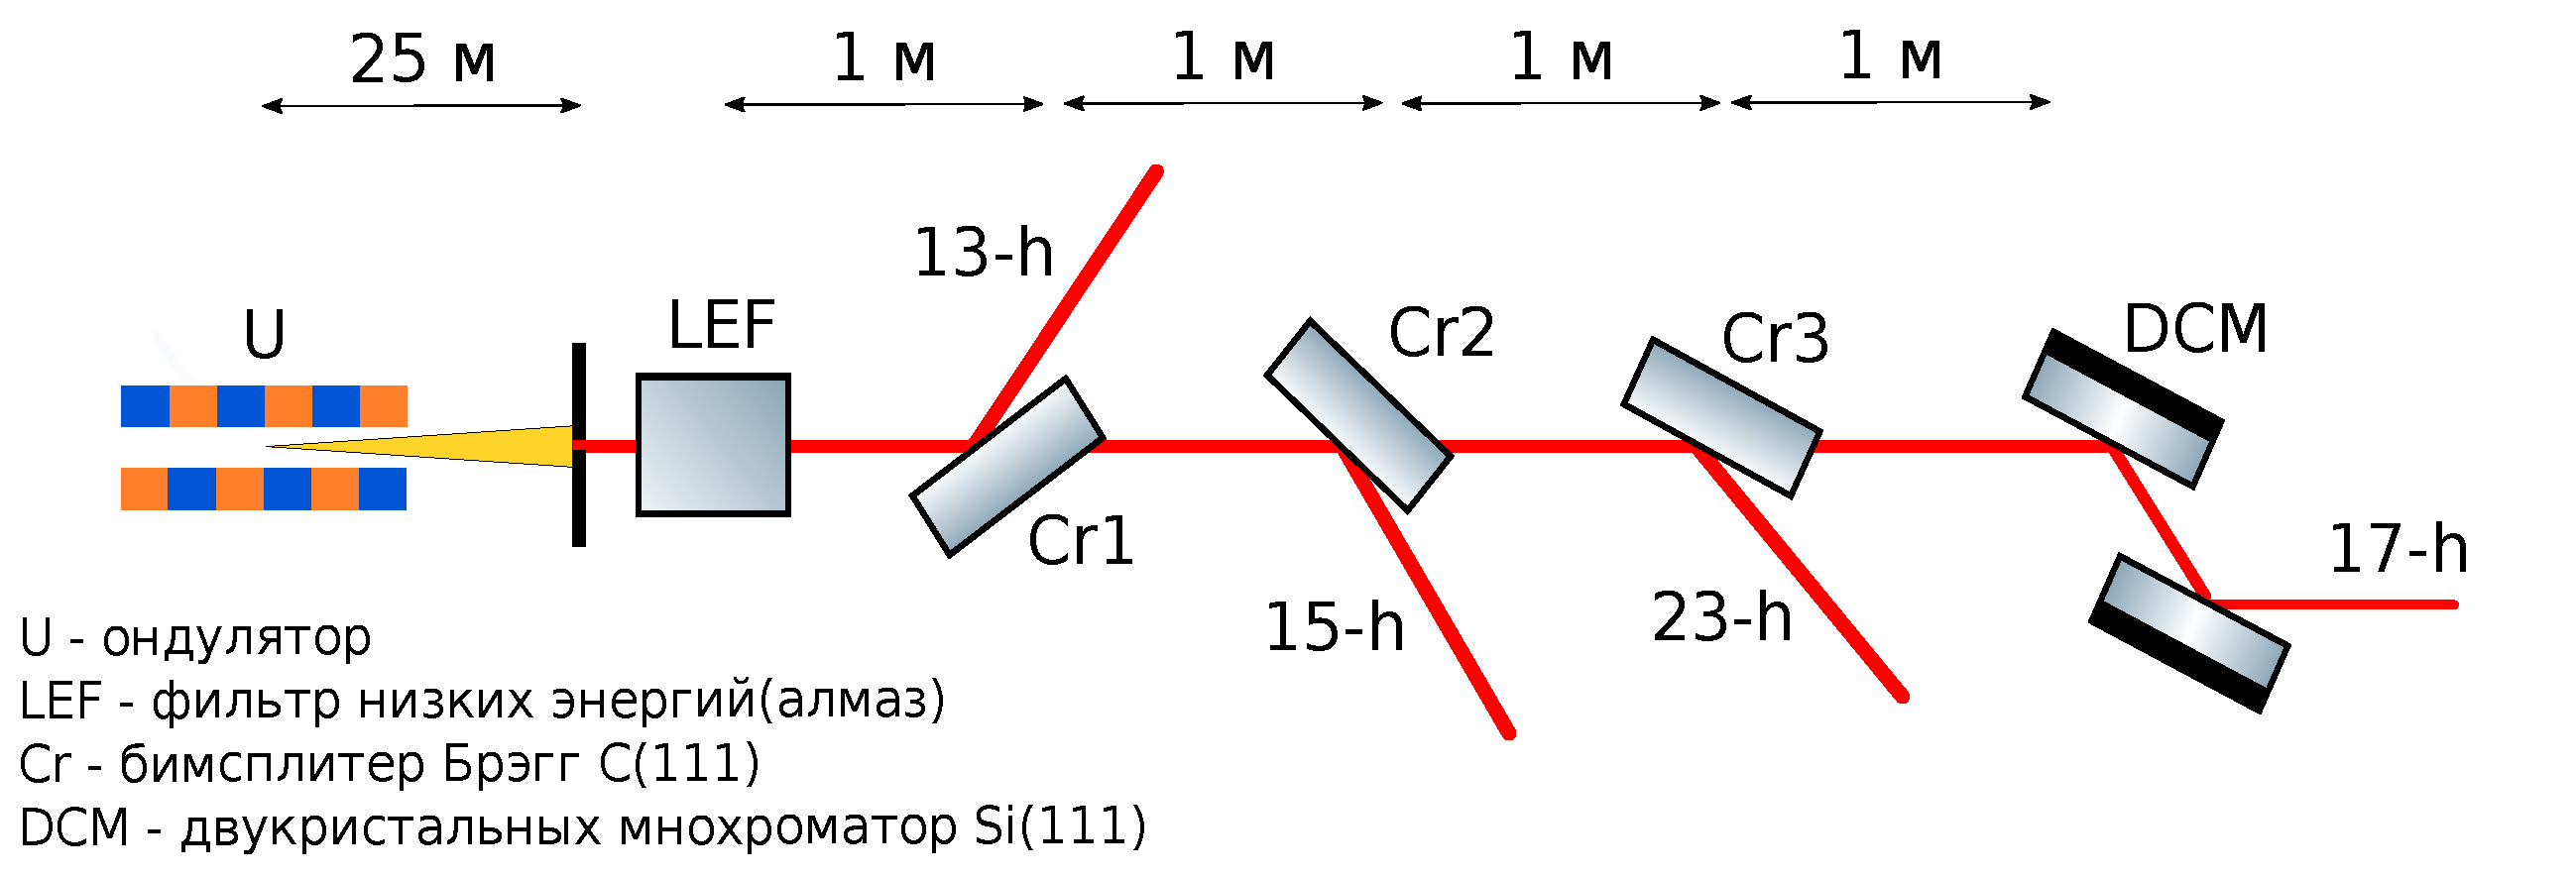
\includegraphics[width=0.8\linewidth]{pic/OptScheme.pdf}}
	%Задача: расчёт тепловых нагрузок в первом приближении
\end{figure}
\vspace{-15pt}
\begin{figure}[h]
	\center{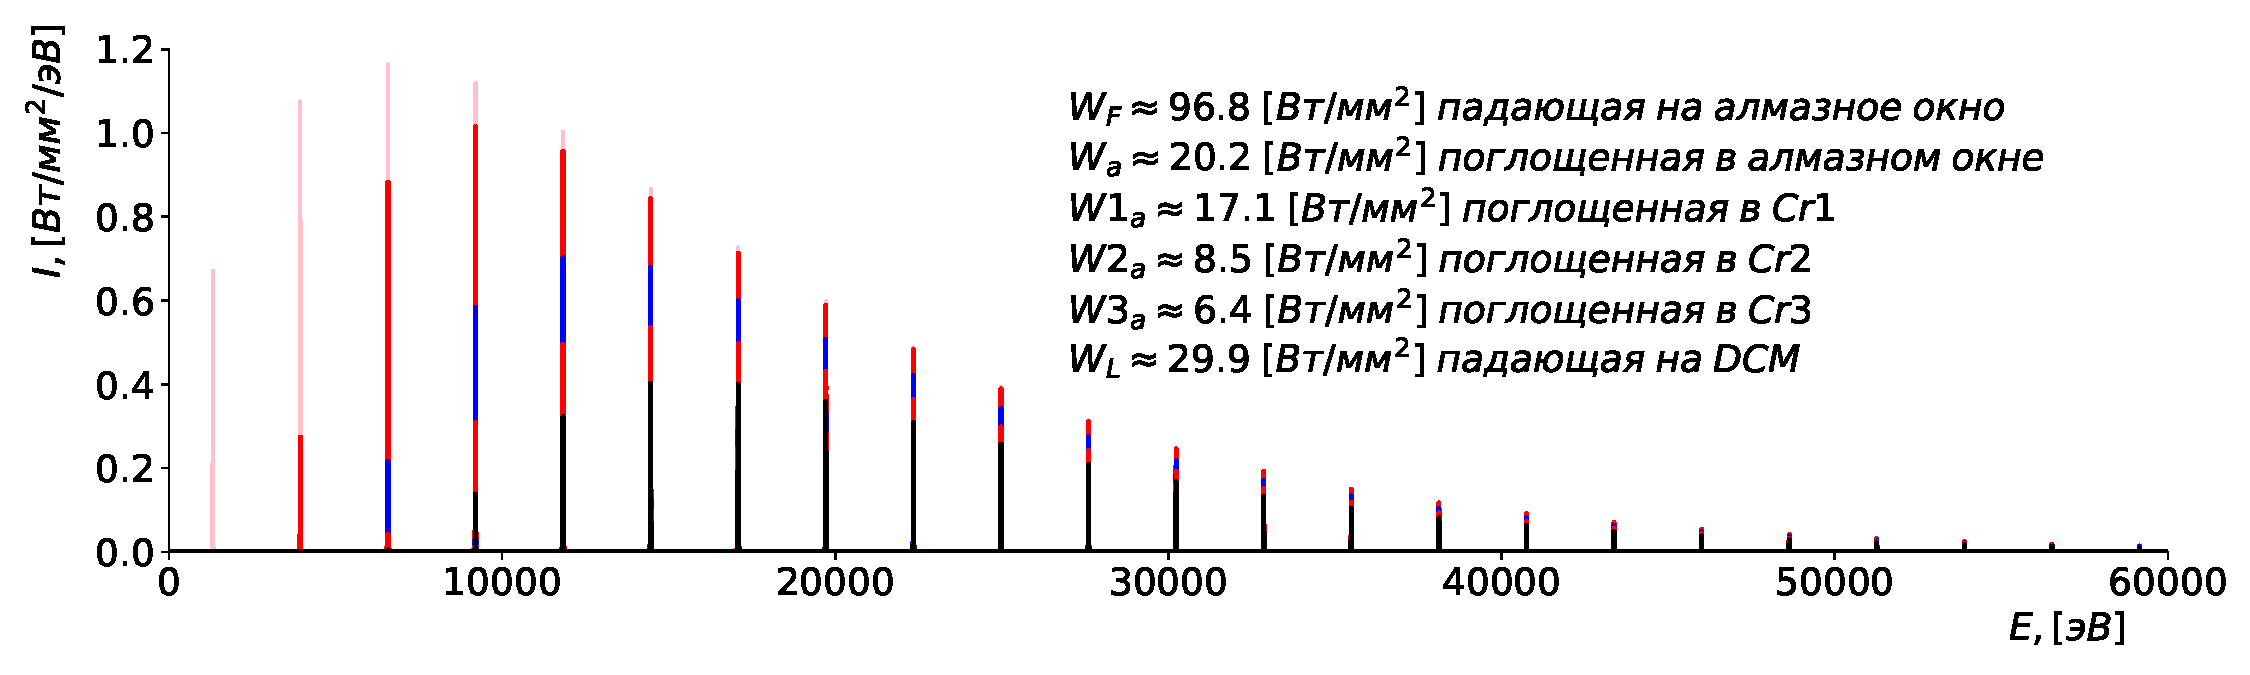
\includegraphics[width=0.99\linewidth]{pic/full_spec.pdf}}
\end{figure}
\tiny{\textit{@Andrei Trebushinin ссылка на \href{https://github.com/TrebAndrew/thesis_andrei.git}{GitHub}}}
\end{frame}

\small
\begin{frame}
\frametitle{Ондулятор станции 1-4 (Quick-XAFS)}\label{t1}
\vspace{-10pt}
\begin{figure}[h]
	\raggedright{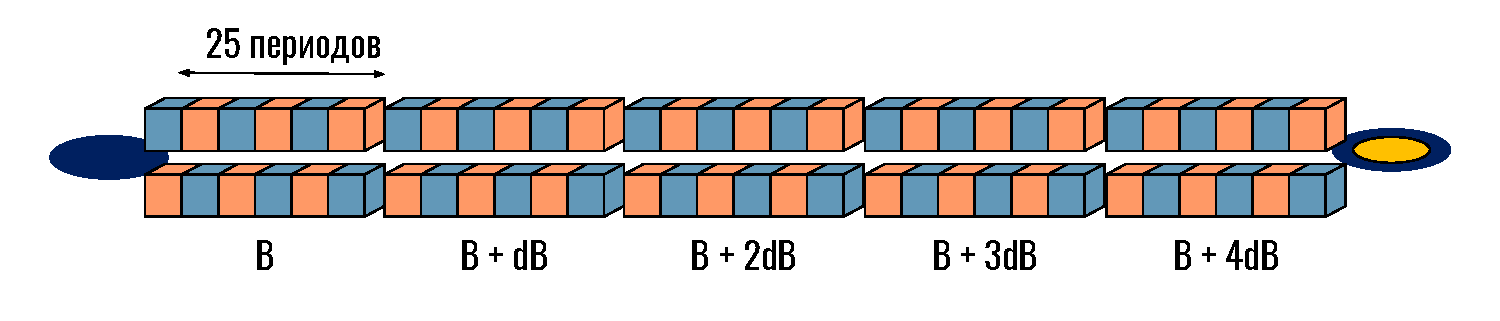
\includegraphics[width=0.99\linewidth]{pic/und.pdf}}
\end{figure}
\vspace{-25pt}
\begin{figure}[h]
	\begin{minipage}[h]{0.49\linewidth}
		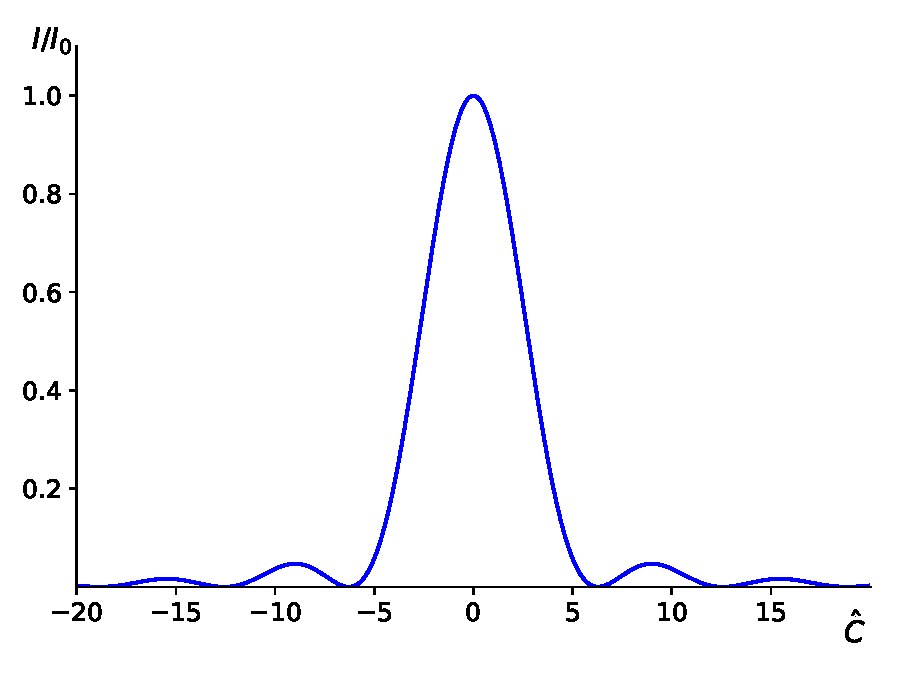
\includegraphics[width=0.99\linewidth]{pic/spec_C.pdf}\\
		\tiny{$\mathnormal{\hat{C} = CL_u = 2\pi N_u\cfrac{\Delta\omega}{\omega_r}}$}
	\end{minipage}	
	\begin{minipage}[h]{0.49\linewidth}
		\begin{itemize}
			\item {Широкий спектр для Quick-XAFS  спектроскопии $\mathnormal{\approx 1}$ $\mathnormal{keV}$}
			\item {$\mathnormal{\cfrac{\Delta \omega}{\omega_{ph}} = \cfrac{\Delta \lambda}{\lambda_{ph}} \sim \cfrac{1}{nL_u}}$}
		\end{itemize}
	\end{minipage}
\end{figure}

\end{frame}

\small
\begin{frame}
\frametitle{Оценки спектра}\label{t1}
\vspace{-5pt}
\begin{figure}[h]
\begin{minipage}[h]{0.49\linewidth}
	\center{Предсказание}
	\vspace{-10pt}
	\center{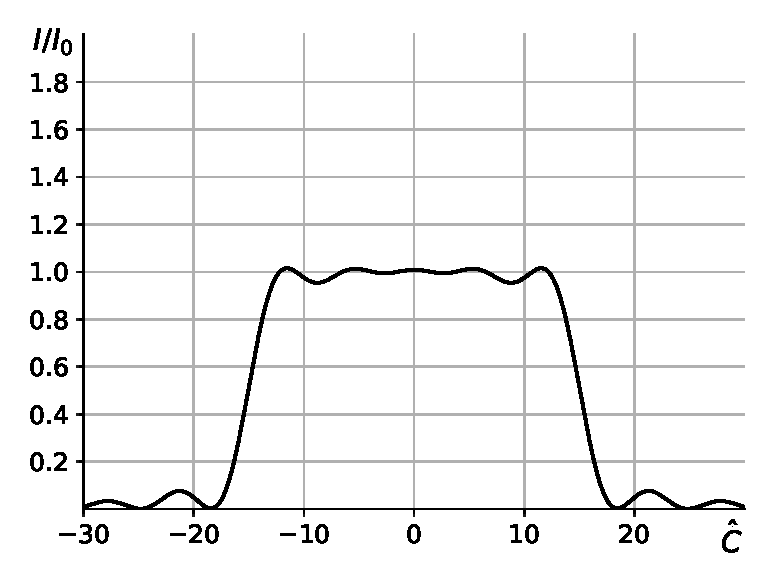
\includegraphics[width=0.99\linewidth]{pic/spec_sinc.pdf}}
\end{minipage}	

\end{figure}
\vspace{-15pt}
\begin{figure}[h]
$\mathnormal{{\widetilde{I}} =
	\bigg(\cfrac{\omega eA_{JJ}}{2c^2 \gamma z_0}\bigg)^2\bigg[
	\displaystyle\sum\limits_{n =-2}^{2}(K_0 + n\Delta K)^2sinc^2(\hat{C_n})}\bigg]$\\

\end{figure}
\end{frame}

\small
\begin{frame}
\frametitle{Моделирование SRW}\label{t1}
\vspace{-36pt}
\begin{figure}[h]
	\begin{minipage}[h]{0.49\linewidth}
		\center{Предсказание}
		\vspace{-10pt}
		\center{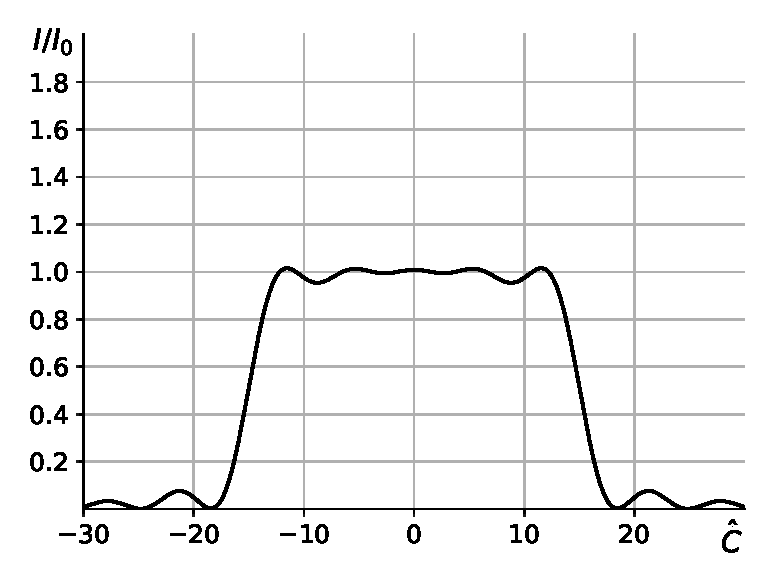
\includegraphics[width=0.99\linewidth]{pic/spec_sinc.pdf}}
	\end{minipage}	
	\begin{minipage}[h]{0.49\linewidth}
		\center{Симуляция SRW}
		\vspace{-10pt}
		\center{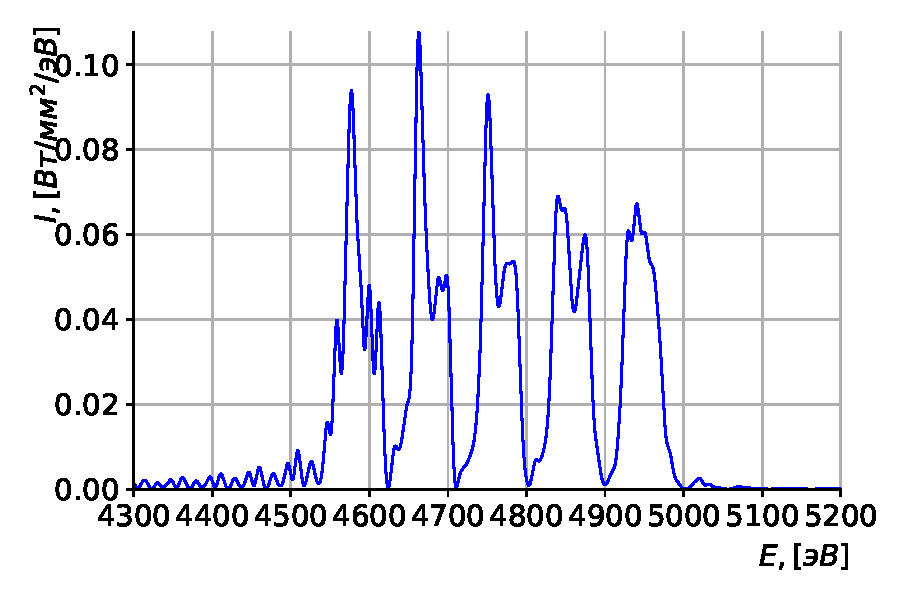
\includegraphics[width=0.99\linewidth]{pic/sim_und_spec.pdf}}
	\end{minipage}
\end{figure}
\vspace{-30pt}
\begin{figure}[h]
	\center{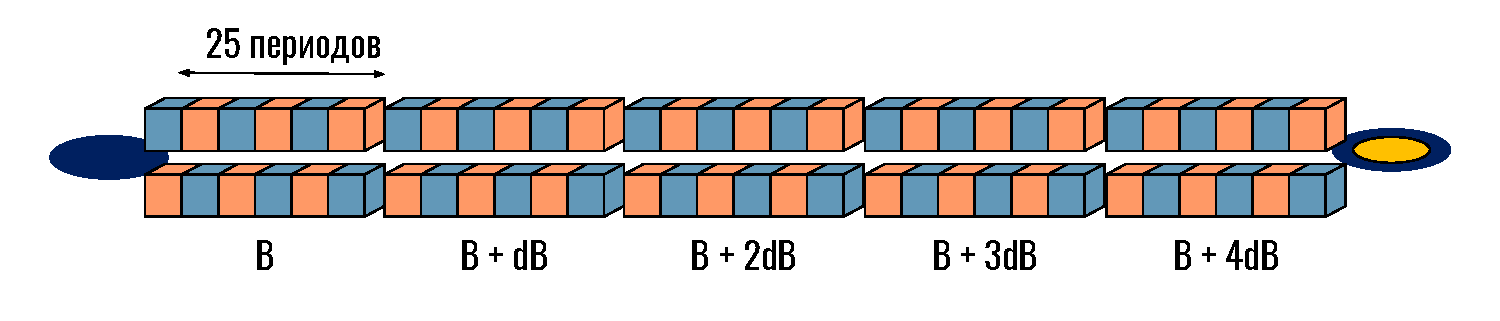
\includegraphics[width=0.7\linewidth]{pic/und.pdf}}
\end{figure}
\end{frame}

\small
\begin{frame}
\frametitle{Интерференция в спектре}\label{t1}
\vspace{-5pt}
\begin{figure}[h]
	\begin{minipage}[h]{0.49\linewidth}
		\center{Аналитический результат}
		\vspace{-10pt}
		\center{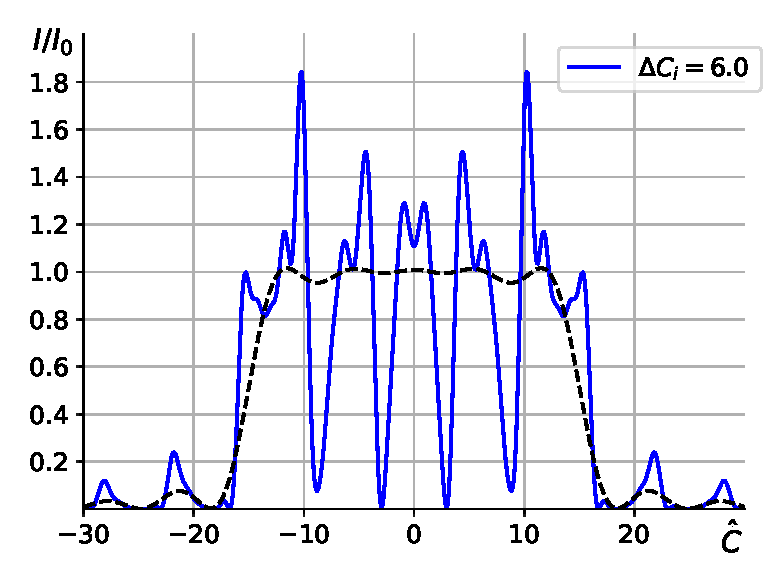
\includegraphics[width=0.99\linewidth]{pic/spec_from_sec_und.pdf}}
	\end{minipage}	
	\begin{minipage}[h]{0.49\linewidth}
		\center{Симуляция SRW}
		\vspace{-10pt}
		\center{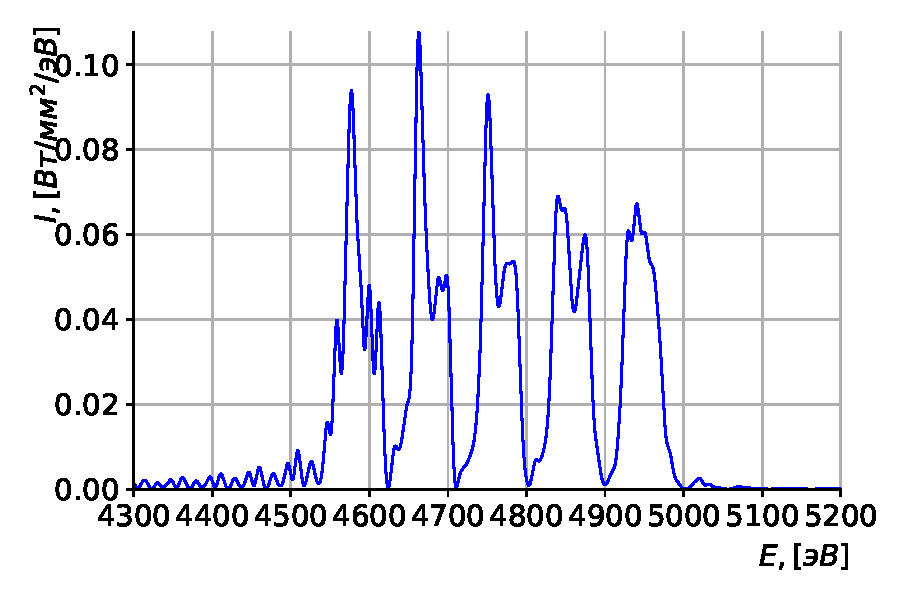
\includegraphics[width=0.99\linewidth]{pic/sim_und_spec.pdf}}
	\end{minipage}
\end{figure}
\vspace{-20pt}
\begin{figure}[h]
	$\mathnormal{{\widetilde{I}} =
		\bigg(\cfrac{\omega eA_{JJ}}{2c^2 \gamma z_0}\bigg)^2\bigg[
		\textcolor{gray}{\displaystyle\sum\limits_{n =-2}^{2}(K_0 + n\Delta K)^2\sinc^2(\hat{C_n}) + }}$\\
	
	$\mathnormal{\displaystyle\mathop{\sum\limits_{n, m =-2}^{2}}_{n \neq m}K^2_0\bigg(1 + n\cfrac{\Delta K}{K_0} + m\cfrac{\Delta K}{K_0}\bigg)
	\textcolor{violet}{\sinc^2(\hat{C_n})e^{i(n-m)\hat{C}_0 + (n^2 - m^2)\Delta \hat{C}}}\bigg]}$
\end{figure}
\end{frame}

\small
\begin{frame}
\frametitle{Планы}\label{t1}
\begin{center}
	\begin{itemize}
		\item Детальное моделирование оптических схем
		\item Принятие решения по концепции ондулятора станции 1-4	
	\end{itemize}
\end{center}
{\textit{\href{https://github.com/TrebAndrew/thesis_andrei.git}{Здесь} можно следить за работой оптической группы}}\\
{\textit{\href{https://github.com/TrebAndrew/diploma.git}{Здесь} за текстом дипломной работы}}\\
{\textit{Моя почта: $trebandrej@gmail.com$}}\\
\end{frame}

\begin{frame}
\begin{center}
	\textbf{Благодарю за внимание}
\end{center}
\end{frame}

\end{document}
